\documentclass[11pt,a4paper]{ivoa}
\input tthdefs
\usepackage{verbatim}
\usepackage{longtable}
\usepackage{tabularx}
\usepackage{todonotes}
\usepackage{textcomp}
\usepackage{listings}
\lstloadlanguages{SQL, SPARQL}    
\lstset{flexiblecolumns=true,stringstyle=\ttfamily,showstringspaces=False}

\title{Using Wikidata for an Observation Facility Vocabulary}

% see ivoatexDoc for what group names to use here; use \ivoagroup[IG] for
% interest groups.
\ivoagroup{Semantics}

\author[mailto:baptiste.cecconi@obspm.fr]{Baptiste Cecconi}
\author{Laura Debisschop}
\author{Mireille Louys}
\author{Emmanuelle Perret}
\author{Markus Demleitner}

\editor{Baptiste Cecconi}

% \previousversion[????URL????]{????Concise Document Label????}
\previousversion{This is the first public release}

   
  
\begin{document}
\begin{abstract}
This document presents how Wikidata can be used for defining a 
vocabulary for Observation Facilities. 
\end{abstract}


\section*{Acknowledgments}

This work has been developed by the VESPA (Virtual European Solar
and Planetary Access) team.  VESPA has been designed in the frame of
Europlanet 2020 Research Infrastructure project and finalised
during the Europlanet 2024 Research Infrastructure project,
based on an assessment phase in the Europlanet Research Infrastructure
 programme, JRA4 work package (IDIS activity).

The Europlanet-RI project was funded by the European Commission under the
7th Framework Program, grant 228319 ``Capacities Specific Programme''.
The Europlanet 2020 Research Infrastructure project has
received funding from the European Union's Horizon 2020 research and
innovation programme under grant agreement No 654208.  The Europlanet-2024
Research Infrastructure project has received funding from
the European Union's Horizon 2020 research and innovation programme under
grant agreement No 871149.  Additional funding was provided in France by
the CNRS / Action Sp\'ecifique Observatoire Virtuel and Programme National
de Plan\'etologie / INSU, as well as CNES, through the participation to
IPDA and IHDEA activities.

\section*{Conformance-related definitions}

The words ``MUST'', ``SHALL'', ``SHOULD'', ``MAY'', ``RECOMMENDED'', and
``OPTIONAL'' (in upper or lower case) used in this document are to be
interpreted as described in IETF standard RFC2119 \citep{std:RFC2119}.

The \emph{Virtual Observatory (VO)} is a
general term for a collection of federated resources that can be used
to conduct astronomical research, education, and outreach.
The \href{https://www.ivoa.net}{International
Virtual Observatory Alliance (IVOA)} is a global
collaboration of separately funded projects to develop standards and
infrastructure that enable VO applications.


\section{Introduction}

Searching for data products using the observation facility is a 
typical use case for the VO, e.g.: \emph{Find Hubble observations
of Saturn in Nov.\ 1997}. The two IVOA data discovery interfaces, 
ObsTAP \citep{2017ivoa.spec.0509L} and EPN-TAP \citep{ivoa:epntap}, 
include keywords allowing such queries (with keywords like 
\texttt{facility} or \texttt{instrument\_host\_name}). However, with 
the specific previous example, a query on EPN-TAP will not show any 
result, since the available data are registered with an 
\texttt{instrument\_host\_name} set to \emph{HST}. It is up to the 
data provider to provide observation facility names that likely match
users' ideas of their designations.  Since
observation facility names usually have acronyms, aliases or alternate 
names, which may further depend the context or even on 
time (e.g., space mission can change name when they are extended), this
is certainly no easy task.

In order to address this use case, two steps are required: (a) group
all known aliases for each observation facilities in a lookup table, 
which can be used to build a dedicated name resolver service; and 
(b) propose a vocabulary to be used in new data in order to restrict the
need for the name resolver to the data discovery clients.
This document does not address another key
aspect of observation facilities in the VO, which is their 
description with a dedicated information model and standardised 
metadata.

In this document, we first describe the selected semantical scope of 
observation facilities in this Note. We then present the various 
lists of observation facility names that are available. We expose the 
use of Wikidata as a reference knowledge base. We finally propose a 
vocabulary scheme based on this study. 

\subsection{Role within the VO Architecture}

\begin{figure}
\centering

% As of ivoatex 1.2, the architecture diagram is generated by ivoatex in
% SVG; copy ivoatex/archdiag-full.xml to role_diagram.xml and throw out
% all lines not relevant to your standard.
% Notes don't generally need this.  If you don't copy role_diagram.xml,
% you must remove role_diagram.pdf from SOURCES in the Makefile.

\includegraphics[width=0.9\textwidth]{role_diagram.pdf}
\caption{Architecture diagram for this document}
\label{fig:archdiag}
\end{figure}

Fig.~\ref{fig:archdiag} shows the role this document plays within the
IVOA architecture \citep{2010ivoa.rept.1123A}.

\section{Observation Facility Semantic Scope}
\label{sec:scope}

Several groups have been working on modelling the roles and 
relationships between elements of measurement or observation devices. 
Appendix \ref{appendix:models} presents the main models currently 
available. 

In this document, we use a definition close to that of SPASE 
(see Section \ref{appendx:models:spase}), that is: an 
\emph{observation facility} is an apparatus bearing one or several 
instruments (measuring devices, modelling codes, etc.), which is 
can be defined with a location, or a set of locations. In that sense, we deal with observatories, 
telescopes in observatories, spacecraft, space probes, space missions 
(as a group of spacecraft), etc. We also include laboratories or 
facilities conducting  experiments, such as supporting observation on 
ices, plasma, gases, etc., as well as planetary analogue sites. The 
instruments (which are defined by their method or type of observation) 
attached to or mounted on the observation facilities are out of the scope 
of this study.


\section{Observation Facility Lists}
Many observation facility lists are available in several contexts. Each list
defines names and/or identifiers for each element. We present here the main 
lists that we have identified and processed during the study. The various 
lists (as available at the time of writing) are available (in raw or 
processed format) on: \url{https://github.com/epn-vespa/FacilityList}.
Table \ref{tab:lists} shows the record count for each of the lists. 
Example records are also available in Appendix \ref{appendix:lists}. 


\begin{table}
\caption{Observation Facility name lists, with their scope and record 
count at the time of writing.}\label{tab:lists}
\begin{tabular}{lll}
List Name               & Scope           & Record Count \\
\hline
NSSDC                   &           space & 1571 \\
NASA/NAIF               &           space & 307 \\
NASA/PDS                &           space & 228 \\
SPASE                   & ground \& space & 215 \\
SANA                    &           space & 1513 \\
AAS                     & ground \& space & 563 \\
ADS/Harvard             & ground \& space & 256 \\
IRAF                    & ground          & 28 \\
IAU/MPC                 & ground \& space & 2335 \\
Xephem                  & ground          & 461 \\
WMO/Oscar               &           space & 683 \\
WISERep (telescopes)    & ground          & 108 \\
Astroweb                & ground \& space & 375 \\
Quaero/IMCCE            &           space & 19855
\end{tabular}
\end{table}


\subsection{AAS (American Astronomical Society)}
The AAS is maintaining a \emph{Facility Keyword} list, which should be used
together with their \emph{AASTeX} package. The list includes a keyword 
(short name), the full facility name, the facility location (continent or 
space), the observation wavelength ranges and facility type flags.  

\subsection{ADS (Astronomy Data System)}
The ADS used to propose a list of facilities\footnote{A copy is available here: 
\protect\url{https://github.com/epn-vespa/FacilityList/blob/master/data/ADS/ADS_facilities.txt}}, 
with its former web user interface. The current version of ADS is not using 
such a curated list. The list contains an identifier and a full name. For 
ground based observatories, the identifier is composed of pair of 
short names (observatory and telescope), separated by a \texttt{.} (dot) 
character. For spacecraft, the identifier starts with \texttt{Sa.} and is 
followed by a spacecraft short name.

\subsection{Astroweb}
The Astroweb list\footnote{The latest version is distributed by CDS: 
\protect\url{http://cdsweb.u-strasbg.fr/astroWeb/astroweb/telescope.html}} 
has not been maintained since 2010.  
It still contains information valuable for our present endeavour.
Each record is composed of a full name, an identifier, a long description
a web URL and a set of metadata describing the facility (\emph{high\_energy}, 
\emph{optical}, \emph{solar}, \emph{space}...)

\subsection{IAU-MPC (International Astronomical Union -- Minor Planet Center)}
The IAU-MPC observatory code list\footnote{\protect\url{https://www.minorplanetcenter.net/iau/lists/ObsCodes.html}}
references observatories used for minor planet and solar system small bodies
science, which includes most of the ground based observatories operating in 
optical and infrared. Each record is composed of an identifier (observatory
code), a location on Earth, and a name. In case of spacecraft, the location
coordinates are replaced by \texttt{x} characters.

\subsection{IRAF (Image Reduction and Analysis Facility)}
IRAF is an astronomical data analysis software. It contains a list of 
observation facilities\footnote{\protect\url{http://tdc-www.harvard.edu/iraf/rvsao/bcvcorr/obsdb.html}}.
Each record is composed of an identifier, a full name, a location and 
a timezone identifier. 


\subsection{NASA/NAIF (Navigation and Ancillary Information System)}
The NASA/NAIF team is maintaining orbital and pointing information for 
space missions, using the NASA/SPICE library. The NAIF toolkit includes
several nomenclatures composed of pairs of identifier (numeric) and 
names. In the frame of this study, the NAIF list of spacecraft\footnote{\protect\url{https://naif.jpl.nasa.gov/pub/naif/toolkit_docs/FORTRAN/req/naif_ids.html\#Spacecraft}}, and ground 
stations\footnote{\protect\url{https://naif.jpl.nasa.gov/pub/naif/toolkit_docs/FORTRAN/req/naif_ids.html\#Ground\%20Stations.}}
have been explored.

\subsection{NSSDC (National Space Science Data Centre)}
The NSSDC is a common NASA data centre for space sciences. They maintain a 
list of spacecraft and space platforms grouped by sub-discipline. We have 
used the \emph{Astronomy}, \emph{Planetary-Science} and \emph{Space-Physics} 
lists. The records include an identifier (most usually, this is its 
COSPAR-ID) and a name.

\subsection{NASA/PDS (Planetary Data System)}
The NASA/PDS is the NASA Planetary Science archive, built upon the 
PDS4-IM. As detailed in section \ref{sec:scope}, it is storing 
observation facility metadata into \emph{Context Products}. In this 
study we have analysed the \texttt{airborne}, \texttt{facility},  
\texttt{instrument\_host} and \texttt{telescope}. Each record is 
a PDS4-IM product, many metadata, including a PDS4 Logical 
identifier, and a full name.

\subsection{SANA (Space Assigned Numbers Authority)}
The SANA is managing registries related to space systems, in 
coordination with CCSDS (Consultative Committee for Space Data
Systems). The \emph{Spacecraft Identifier} registry gathers many
spacecraft metadata but mostly concerning the telemetry and 
telecommand (TMTC) links. We have only used the 
spacecraft identifier and name.  

\subsection{Xephem}
Xephem is an astronomical ephemeris and planetarium software. It
contains a list of observatories, available from its Github 
repository\footnote{\url{https://github.com/XEphem/XEphem/blob/main/GUI/xephem/auxil/xephem_sites}}.
Each record includes of a name.
  
\subsection{WISeREP (Weizmann Interactive Supernova Data Repository )}
The WISeREP facility includes lists\footnote{\url{https://www.wiserep.org/aux}} 
of sites, telescopes and instruments. We have analysed its list of telescope 
in this Note. Each record includes an identifier, a name and a 
nickname.

\subsection{SPASE (Space Physics Archive Search and Extract)} 
The SPASE registry is using the SPASE model \citep{Roberts:2018bi}. 
It contains records of the \emph{Observatory} type, which cover our
scope as explained in section \ref{sec:scope}. The SPASE records 
are stored as XML trees, and are available from the HPDE (Heliophyiscs
Data Environment) Github repository\footnote{\url{https://github.com/hpde}},
which is organised by \emph{Naming Authority}. Although each naming 
authority may have an Observatory section, most of the Observatory 
records are currently registered in the SMWG (SPASE Metadata Working
Group) repository\footnote{\url{https://github.com/hpde/SMWG}}.
Each observatory records includes an identifier (SPASE URI) and a name. 

\subsection{WMO/Oscar (World Meteorologic Organisation/Observing Systems Capability Analysis and Review Tool)}
The OSCAR tool of the WMO is maintaining several lists concerning
observation facilities, with Space-based resources\footnote{\url{https://space.oscar.wmo.int/spacecapabilities}}, 
as well as ground based stations\footnote{\url{https://oscar.wmo.int/surface/\#/}}. 
We consider these lists since Space Weather (or Space Situational 
Awareness) is part of both the WMO and IVOA scopes. The analysis of these 
resources requires filtering to keep only those within the IVOA scope.  
Each satellite record includes an acronym, and a full name.  

\subsection{IMCCE/Quaero (Institut de M\'ecanique C\'eleste et de Calcul des \'Eph\'em\'erides)}
The IMCCE lab is proposing a name resolver\footnote{\url{https://ssp.imcce.fr/webservices/ssodnet/api/quaero/}} 
using its SsODNet (Solar system Open Database Network) service. This
service, called \emph{Quaero} contains several types of records. Using 
the query \url{https://api.ssodnet.imcce.fr/quaero/1/sso/search?q=type:Spacecraft}, 
it is possible to access to the list of Spacecraft records. Each 
record is includes of an identifier, a name, and a list of
aliases.

\subsection{Wikidata}
Wikidata is a free and open knowledge base, community curated, and 
based on structured data following the W3C's Resource Description
Framework RDF. The record content is not 
constrained by a detailed information model. Each record is 
composed of a language-neutral identifier, a human-readable title, 
and a set of human-readable aliases in several 
languages. It also has a set of \emph{statements}, composed of properties
(e.g., \emph{is instance of}) linked to a value (e.g., \emph{space 
observatory}), and a set of \emph{external identifiers}. Observation 
facilities are retrieved using a set of record classes (\emph{is 
instance of} statement). 

\section{More details on Wikidata}
Mapping the lists of names and identifiers presented in the previous
section is a cumbersome task, requiring a lot of time, effort and 
curation on the long run. After the assessment of the various lists,
it appears that Wikidata records contain most of the information 
required for the name resolver use case: the title, aliases and 
external identifiers are accurate for most of the studied records. 

We present below a few examples showing the various cases, with the 
relevant subset of metadata available in the records.

\noindent\begin{longtable}{p{.2\textwidth}p{.75\textwidth}}
\hline
\hline
\multicolumn{2}{l}{\bf Example 1. Hubble Space Telescope}\\
\hline
URI        & \url{https://www.wikidata.org/wiki/Q2513}\\
Label      & Hubble Space Telescope \\
Aliases    & HST, Hubble, Hubbleteleskop, t\'elescope Hubble, Telescopio Espacial Hubble, TEH, telescopio spaziale Hubble, etc\\
\multicolumn{2}{c}{\sl selected statements}\\
is-a & space observatory \\
\multicolumn{2}{c}{\sl selected identifiers}\\
COSPAR ID  & 1990-073B \\
NSSDCA ID  & 1990-073B \\
IAU-MPC ID & 250\\
NAIF ID    & -48\\
UAT ID     & 761\\
SCN ID     & 20580 \\
\hline
\hline
\multicolumn{2}{l}{Example 2. Venera 2}\\
\hline
URI & \url{https://www.wikidata.org/wiki/Q719617}\\
label      & Venera 2\\
Aliases    & 3MV-4 No.4, etc\\
\multicolumn{2}{c}{\sl selected statements}\\
is-a & space probe \\
is-a & 3MV (Soviet unmanned probe design) \\
is-part-of     & Venera \\
\multicolumn{2}{c}{\sl selected identifiers}\\
COSPAR ID  & 1965-091A \\
NSSDCA ID  & 1965-091A \\
SCN ID     & 01730 \\
\hline
\hline
\multicolumn{2}{l}{Example 3. Mount Wilson Observatory}\\
\hline
URI & \url{https://www.wikidata.org/wiki/Q466863}\\
Label      & Mount Wilson Observatory\\
Aliases    & Observatoire du Mount Wilson, Mount Wilson, Mount-Wilson-Observatorium, Osservatorio di Mount Wilson, etc.\\
\multicolumn{2}{c}{\sl selected statements}\\
is-a & astronomical observatory \\
\multicolumn{2}{c}{\sl selected identifiers}\\
ISNI       & 0000 0001 2168 8877\\
IAU-MPC ID & 672\\
ROR ID     & 03xvqcz58\\
\hline
\hline
\multicolumn{2}{l}{Example 4. SOHO}\\
\hline
URI & \url{https://www.wikidata.org/wiki/Q320638}\\
label      & Solar and Heliospheric Observatory\\
Aliases    & SOHO, Sonde SOHO, Solar Heliospheric Observatory, Observatorio Solar y Heliosferico, etc.\\
\multicolumn{2}{c}{\sl selected statements}\\
is-a & space observatory \\
\multicolumn{2}{c}{\sl selected identifiers}\\
COSPAR ID  & 1995-065A \\
NSSDCA ID  & 1995-065A \\
IAU-MPC ID & 249\\
NAIF ID    & -21\\
SCN        & 23726\\
\hline
\hline
\multicolumn{2}{l}{Example 5. COBE}\\
\hline
URI & \url{https://www.wikidata.org/wiki/Q49445}\\
Label      & Cosmic Background Explorer\\
Aliases    & COBE, Explorer 66, etc.\\
\multicolumn{2}{c}{\sl selected statements}\\
is-a & space observatory \\
is-a & cosmic microwave background experiment \\
\multicolumn{2}{c}{\sl selected identifiers}\\
COSPAR ID  & 1989-089A \\
NSSDCA ID  & 1989-089A \\
SCN        & 20322\\
\hline
\hline
\multicolumn{2}{l}{Example 5. CFHT}\\
\hline
URI & \url{https://www.wikidata.org/wiki/Q1031946}\\
Label      & Canada-France-Hawaii Telescope\\
Aliases    & observatoire Canada-France-Hawa\"i, T\'elescope Canada-France-Hawaii, Tcfh, etc.\\
\multicolumn{2}{c}{\sl selected statements}\\
is-a & astronomical observatory \\
is-a & optical telescope \\
is-part-of & Mauna Kea Observatories\\
\multicolumn{2}{c}{\sl selected identifiers}\\
ISNI       & 0000 0004 0601 3064\\
ROR ID     & 05xq4gr47 \\
\hline
\hline
\multicolumn{2}{l}{Example 6. EHT}\\
\hline
URI & \url{https://www.wikidata.org/wiki/Q3944788}\\
Label      & Event Horizon Telescope\\
Aliases    & EHT\\
\multicolumn{2}{c}{\sl selected statements}\\
is-a & very-long-baseline interferometry \\
is-a & research collaboration \\
has-part & Atacama Large Millimeter Array\\
has-part & Atacama Pathfinder Experiment\\
has-part & IRAM 30-meter telescope\\
has-part & James Clerk Maxwell Telescope\\
has-part & Large Millimeter Telescope\\
has-part & Submillimeter Array\\
has-part & Heinrich Hertz Submillimeter Telescope\\
has-part & South Pole Telescope\\ 
\multicolumn{2}{c}{\sl selected identifiers}\\
ISNI       & 0000 0004 0601 3064\\
ROR ID     & 05xq4gr47 \\
\hline
\end{longtable}


Wikidata can be updated to improve the quality of the knowledge.
Within the scope of this work, this implies three types of updates:
\begin{itemize}
\item added relevant \emph{is instance of} statements, to ease the 
record discovery and limit the complexity of the queries (see, e.g., 
Appendix \ref{appendix:sparql}). 
\item include \emph{external identifiers} statements, when values 
are missing
\item define new identifier authorities in Wikidata for lists that 
are not yet registered to be used as \emph{external identifiers}. 
\end{itemize}
The first two items are easy to set up and solve when the record is 
found. However, if the object of the \emph{is instance of} statement is 
not set as expected, finding the record is not always 
straightforward, since common names in instrument designations 
can be used in many other contexts. 
The latter item (defining new \emph{external identifiers}) is 
possible through a process\footnote{\url{https://www.wikidata.org/wiki/Wikidata:Property_proposal/Authority_control}}
defined by Wikidata. 

\section{A Name Resolver for Observation Facilities}
Using the Wikidata knowledge base, it is possible to build a name
resolver for observation facilities. A prototype is planned that would
in regular intervals retrieve the relevant 
Wikidata content using queries similar to the one
given in Appendix \ref{appendix:sparql}. This query provides
a JSON document that can be easily ingested into an elastic-search
data base (or similar) to set a name resolver very similarly to 
the Quaero service of IMCCE. 

\section{A Vocabulary for Observation Facilities}
An observation facility vocabulary could be built using Wikidata
as an external knowledge base, similarly to the \emph{IVOA-flavoured 
UAT} vocabulary\footnote{\url{https://www.ivoa.net/rdf/uat}}.

The internal Wikidata identifier would be hidden to the user, which 
would use the record title as a human readable identifier (with the 
same transformation as for the UAT: lower-cased and hyphen-split). 
Using the same examples as in the previous section we would have: 
\begin{itemize}
\item Q2513: hubble-space-telescope
\item Q719617: venera-2
\item Q466863: mount-wilson-observatory
\item Q320638: solar-and-heliospheric-observatory
\item Q49445: cosmic-background-explorer
\item Q1031946: canada-france-hawaii-telescope
\item Q3944788: event-horizon-telescope
\end{itemize}
In order to build such a list, there is a need to build a Wikidata 
query, which select the records of interest for our purpose.

However, the current limitation of this solution is the heterogeneous 
quality of the statements in Wikidata. The \emph{is-part-of} 
statements will be reused in the IVOA-flavoured Wikidata Observation 
Facility vocabulary to create links between records. A few examples of 
\emph{part of} and \emph{has part} relations are shown below:
{\small \noindent\begin{longtable}{p{.35\textwidth}p{.65\textwidth}}
\textbf{Label} & \textbf{Relations}\\
\hline
\hline
venera-2  & \emph{is-part-of} venera\\
\hline
mount-wilson-observatory & \emph{has-part} chara-array\\
                         & \emph{has-part} infrared-spatial-interferometer\\
                         & \emph{has-part} hocker-telescope\\
                         & \emph{has-part} 60-inch-telescope\\
                         & \emph{has-part} 150-foot-solar-tower\\
\hline
canada-france-hawaii-telescope & \emph{is-part-of} mauna-kea-observatories\\
\hline
event-horizon-telescope & \emph{has-part} atacama-large-millimeter-array\\
                        & \emph{has-part} atacama-pathfinder-experiment\\
                        & \emph{has-part} iram-30-meter-telescope\\
                        & \emph{has-part} james-clerk-maxwell-telescope\\
                        & \emph{has-part} large-millimeter-telescope\\
                        & \emph{has-part} submillimeter-array\\
                        & \emph{has-part} heinrich-hertz-submillimeter-telescope\\
                        & \emph{has-part} south-pole-telescope\\
\hline
european-vlbi-network   & \emph{has-part} effelsberg-100-m-radio-telescope\\
                        & \emph{has-part} westerbork-synthesis-radio-telescope\\
                        & \emph{has-part} lovell-telescope\\
                        & \emph{has-part} cambridge-merlin-telescope\\
                        & \emph{has-part} mark-ii\\
                        & \emph{has-part} medicina-32-m-radio-telescope\\
                        & \emph{has-part} onsala-space-observatory-20-m-telescope\\
                        & \emph{has-part} onsala-space-observatory-25-m-telescope\\
                        & \emph{has-part} noto-32-m-radio-telescope\\
                        & \emph{has-part} torun-rt4\\
                        & \emph{has-part} metsahovi-14m-radio-telescope\\
                        & \emph{has-part} sheshan-25m-radio-telescope\\
                        & \emph{has-part} nanshan-radio-telescope\\
                        & \emph{has-part} yebes-observatory-rt40m\\
                        & \emph{has-part} wettzell-20m-radio-telescope\\
                        & \emph{has-part} madrid-deep-space-communication-complex\\
                        & \emph{has-part} hartebeesthoek-radio-astronomy-observatory\\
                        & \emph{has-part} arecibo-radio-telescope\\
\hline
\end{longtable}}

\section{Discussion}
This note presents how to use Wikidata to setup a name resolver 
for Observations Facilities, and it should be possible to setup 
an Observation Facility vocabulary using the same knowledge base.

As stated in the introduction, this note is not addressing the 
information model required to describe observation facilities. 
Such modelling effort should be done to formalise the metadata 
associated to the observation facilities, as well as linking 
with associated instruments. The work done by the NASA/PDS4 or
SPASE groups will be very helpful to start this effort. 

The introduction also stated that the instruments mounted or 
associated to the observation facilities were not in the scope
of the note. There are fewer openly accessible resources
listing instruments than for observation facilities, and 
Wikidata is highly incomplete for links between observation facilities
and instruments; in addition, many instruments
are not yet present in Wikidata.

However is it important to understand the community engagement 
underlying Wikidata is a strength as much as a weakness. The 
general public engagement allows to have a very complete  
knowledge base, with regularly curated records and links. However
there is no coordination for the curation nor for the consistency
of the properties used for linking resources. Each contributor may
have his own views on the way to link resources, and they may not 
agree to update their resource-linking scheme to the IVOA use-case.
Indeed, we have encountered difficulties to find a query allowing 
to retrieve a clean set of resources for our purpose. We worked on 
Wikidata content, first to curate resources (with success in general), 
and then to update properties or labels to reduce the overhead (with
less success in this case). Some Wikidata contributors kept removing 
our contributions, even after explaining the rationale of the changes. 
Hence, there is a probably a need for an external knowledge base to 
keep track of IVOA-curated resources.  

Finally, the recent RDA \emph{PID for Instruments} 
recommendation\footnote{\url{https://www.rd-alliance.org/node/57186/outputs}} 
covers a scope similar to this note. However, a closer 
assessment of this document logically reveals concepts very 
close to the Datacite schema, and is not really applicable to 
the needs presented here. Furthermore, it is preferable that 
PIDs are maintained by the resource maintainer, so that they 
are timely and adequately curated and updated. 

\appendix
\section{Metadata Models}
\label{appendix:models}

\subsection{IPDA - PDS4 Information Model}
The PDS4-IM (NASA Planetary Data System version 4 Information Model) 
is the NASA planetary science archive underlying information
model. It can be considered as a serialization of the OAIS ---Open 
Archival Information System, \citep{iso:oais}--- model \citep{Hughes:2017bt}.  
It is managed in the frame of the IPDA (International Planetary 
Data Alliance) and is used by the ESA and JAXA planetary science 
archives. 

The PDS4-IM includes terms to describe an \emph{Observing\_System}, see 
Figure \ref{fig:pds4-concept-map}, defined as follows:
``\emph{The Observing System class describes the entire suite used to 
collect the data}''. At the time of writing, the list of 
\texttt{Observing\_System\_Components}\footnote{
\url{https://pds.nasa.gov/datastandards/documents/im/v1/index_1H00.html\#attribute_pds_observing_system_component_pds_type}}
is defined as: ``\emph{Airborne, Aircraft, Artificial Illumination, 
Balloon, Computer, Facility, Host, Instrument, Laboratory, Literature 
Search, Naked Eye, Observatory, Spacecraft, Suborbital Rocket, 
Telescope}'', each of which is defined in the PDS4-IM. 

Every element in the archive system is a product. Observation 
facilities description records are serialised using so-called 
\emph{Context Products}. The PDS4 context
products are currently available online at: 
\url{https://pds.nasa.gov/data/pds4/context-pds4/}. This 
page provides access to context product types like: \emph{facility}, 
\emph{instrument}, \emph{instrument\_host}, \emph{investigation}, 
\emph{telescope}, etc. The \emph{Hubble Space Telescope} 
record\footnote{\protect\url{https://pds.nasa.gov/data/pds4/context-pds4/instrument_host/spacecraft.hst_1.3.xml}} 
is providing a series of metadata, including an identifier, a title, 
a reference, a description, and many internal references to other 
context products registered in the PDS4 database, including 
observed targets, and investigations (observation campaigns), hosted 
instruments, etc.

\begin{figure}
\centering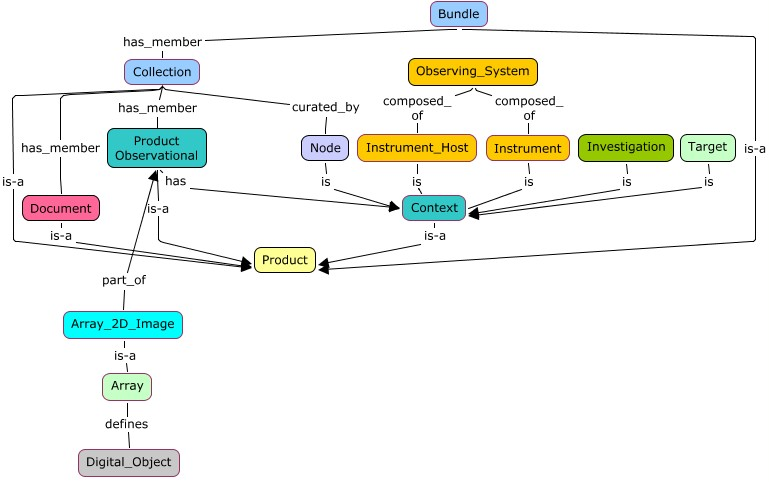
\includegraphics[width=0.9\textwidth]{pds4-concept-map.jpg}
\caption{PDS4 Information Model Concept Map, including the 
\emph{Observing\_System} section. Figure take from PDS4 IM v1.17.0.0 
\protect\citep{pds4-im-v1H00}.}\label{fig:pds4-concept-map}
\end{figure}

\subsection{IVOA -- VOFacility}

The PDS4-IM description has been used to prepare a preliminary study of
an extension of VOResource \citep{2018ivoa.spec.0625P}, called VOFacility, 
which was presented at the ADASS conference in 2015 \citep{Louys:2015to} 
and is available at \url{https://wiki.ivoa.net/internal/IVOA/IvoaSemantics/VOFacility.xsd}. 
This model defines various \emph{observation facility} types: 
\emph{Observatory, Spacecraft, SpaceMission, Telescope, FieldAnalog,
LabExperiment, Simulation}. 


\subsection{OGC - SensorML Model}
In the frame of Earth Observation (EO), the Open Geospatial Consortium
(OGC) has defined a SensorML (Sensor Meta Language) \citep{ogc-sensorml} 
allowing to describe sensors and instruments. One of the application of 
SensorML is the ``\emph{Discovery of sensor, sensor systems, and
processes}.''\footnote{\url{http://wiki.gis.com/wiki/index.php/SensorML}} 
The \emph{PhysicalSystem} type of SensorML is the closest model type to
our observation facility term.  However, it mixes instruments, sensors 
and platform into a single compound type, which does not match our 
typology mapping. 

\subsection{IHDEA - SPASE Model}
\label{appendx:models:spase}
Finally, in the frame of heliophysics, the Space Physics Archive Search
and Extract (SPASE) data model\footnote{Latest version (2.4.0 at the 
time of writing): \url{https://spase-group.org/data/schema/index.html}} 
\citep{Roberts:2018bi,spase-model} has two different
concepts for observatories and instruments: observatories are defined 
with a location (specified either with ground coordinates, or with a 
region in space for spacecraft), whereas instruments are defined with 
a type of measurement. 


\section{List Example Records}
\label{appendix:lists}
\subsection{AAS Record Examples}
\noindent{\tiny\begin{tabularx}{\textwidth}{>{\setlength\hsize{2\hsize}}X|l|>{\setlength\hsize{0.5\hsize}}X|>{\setlength\hsize{0.5\hsize}}X|l|}
Full Name & ID & Location & Wavelengths & Extra type \\
\hline
\hline
3.58m Canada-France-Hawaii Telescope (CFHT) at Mauna Kea Observatory & CFHT & North America and Hawaii & optical, infrared & \\
\hline
Centre National de la Recherche Scientifique (CNRS) 1.93m Telescope at Observatoire de Haute-Provence (OHP)&OHP:1.93m&Europe&optical, infrared& \\
\hline
NASA COsmic Background Explorer satellite mission (also known as Explorer 66)&COBE&Space&infrared, millimeter& \\
\hline
European Space Agency (ESA)/NASA Solar Heliospheric Observatory (SOHO) Satellite Mission&SOHO&Space&ultraviolet, optical& solar
\end{tabularx}}

\subsection{ADS Record Examples}
\noindent{\tiny\begin{tabularx}{\textwidth}{lX}
ID & Full Name \\
\hline
\hline
MK.CFHT   & Mauna Kea/CFHT, Canada-France-Hawaii Telescope\\
\hline
OHP.1.93m & Observatoire de Haute-Provence/1.93 meter Telescope \\
\hline
Sa.COBE   & COBE, COsmic Background Explorer satellite \\
\hline
Sa.SOHO   & SOHO, SOlar Heliospheric Observatory satellite
\end{tabularx}}

\section{Wikidata SPARQL query}
\label{appendix:sparql}
At the time of writing of this note, the following SparQL query
is used to retrieve WikiData records:  
{\tiny
\lstinputlisting[language=SPARQL]{sparql_query.txt}
}
 
\section{Observation Facility names in the IVOA}

Three sets of IVOA services are sharing observation facility names: 
the Registry (in the \texttt{facility} keyword of \texttt{VOResource}), 
ObsTAP services (\texttt{facility} keyword) and EPN-TAP services 
(\texttt{instrument\_host\_name} keyword). Data providers have been 
using non-standard names for observation facilities. For some services 
the \texttt{instrument} or \texttt{instrument\_name} keyword also contains 
observation facility information. In order to retrieve relevant terms, the 
query should retrieve distinct pairs of  \texttt{facility}  and  
\texttt{instrument} names.

Using RegTAP, we can retrieve this information, using the following ADQL queries:

\begin{lstlisting}[language=SQL]
SELECT DISTINCT 
  t1.ivoid AS ivoid, 
  t1.detail_value AS facility, 
  t2.detail_value AS instrument 
FROM rr.res_detail AS t1 
  INNER JOIN rr.res_detail AS t2 
  ON t1.ivoid = t2.ivoid 
WHERE t1.detail_xpath='/facility' 
  AND t2.detail_xpath='/instrument'
\end{lstlisting}

For ObsTAP services, the first request retrieves the list of TAP
servers including \texttt{ivoa.obs\_core} table:

\begin{lstlisting}[language=SQL]
SELECT table_name, access_url, ivoid 
FROM ( 
  SELECT ivoid, table_name 
  FROM rr.res_table 
  WHERE table_name = 'ivoa.obscore'
) AS ivotables
  NATURAL JOIN rr.capability
  NATURAL JOIN rr.interface 
WHERE standard_id = 'ivo://ivoa.net/std/tap' 
  AND intf_role='std'
\end{lstlisting}

Then, the following ADQL queries shall be sent to all TAP server, 
using the list of \texttt{access\_url}. The \texttt{ivoa.obs\_core} 
tables are queried as follows: 

\begin{lstlisting}[language=SQL]
SELECT DISTINCT 
  facility_name AS facility, 
  instrument_name AS instrument 
FROM ivoa.obscore
\end{lstlisting}

Finally for EPN-TAP services, the first request retrieves the list of TAP
servers including \texttt{epn\_core} tables (including several standard-id 
values and erroneous values actually present in the registry): 

\begin{lstlisting}[language=SQL]
SELECT table_name, access_url, ivoid 
FROM ( 
  SELECT ivoid, table_name, table_utype 
  FROM rr.res_table 
  WHERE table_utype LIKE 'ivo://vopdc.obspm/std/epncore%' 
    OR table_utype LIKE 'ivo://ivoa.net/std/epntap#table-2.%' 
    OR table_utype='ivo.//vopdc.obspm/std/epncore#schema-2.0'
  ) AS epntables
NATURAL JOIN rr.capability
NATURAL JOIN rr.interface 
WHERE standard_id = 'ivo://ivoa.net/std/tap' 
  AND intf_role='std'
\end{lstlisting}

Then, the following ADQL queries shall be sent to all TAP server, 
using the list of \texttt{access\_url}. The \texttt{epn\_core} 
tables are queried as follows: 

\begin{lstlisting}[language=SQL]
SELECT DISTINCT instrument_host_name, instrument_name 
FROM <table>
\end{lstlisting}
replacing \texttt{<table>} by the actual table name.


\section{Changes from Previous Versions}

No previous versions yet.  
% these would be subsections "Changes from v. WD-..."
% Use itemize environments.


% NOTE: IVOA recommendations must be cited from docrepo rather than ivoabib
% (REC entries there are for legacy documents only)
\bibliography{localrefs,ivoatex/ivoabib,ivoatex/docrepo}


\end{document}
